\subsection{Graphical user interface}
GUI was written in JavaFX framework.

\subsubsection{Connection with backend}
Connection with backend was realized by execution service methods. Example of service request is in listing \ref{lst:GUIBackendConnector}.

\begin{lstlisting}[breaklines=true, numbers=left, stepnumber=1, label={lst:GUIBackendConnector}, caption={Connection with backend through \textit{userService}}, language=Java]
public void saveButtonOnAction(ActionEvent actionEvent) {
  if(getInitialUser() != null ){
      System.out.println(getDataFromForm().toString());
      userService.updateUserById(getInitialUser().getId(), getDataFromForm());
  }
}
\end{lstlisting}

\subsubsection{Sidebar}
Main navigation element of web app is sidebar. It changes according to logged in user. Each of user type has different set of visible buttons on sidebar. Listing \ref{lst:GUISidebarIsButtonValid} contains id's of buttons and allowed role for each button. 


\begin{lstlisting}[breaklines=true, numbers=left, stepnumber=1, label={lst:GUISidebarIsButtonValid}, caption={Sidebar buttons with allowed user types}]
public Boolean isButtonValidForUserType(String buttonId) {
  if (LoginController.getUser() != null) {
      if (buttonId.equals("findBooksButton")) {
          return LoginController.isReader() || LoginController.isLibrarian();
      }
      if (buttonId.equals("ordersButton")) {
          return LoginController.isReader();
      }
      if (buttonId.equals("manageBooksButton")) {
          return LoginController.isLibrarian();
      }
      if (buttonId.equals("manageOrdersButton")) {
          return LoginController.isLibrarian();
      }
      if (buttonId.equals("allUsersButton")) {
          return LoginController.isAdmin();
      }
      if (buttonId.equals("readersButton")) {
          return LoginController.isAdmin() || LoginController.isLibrarian();
      }
      if (buttonId.equals("reportsButton")) {
          return LoginController.isAdmin();
      }
      if (buttonId.equals("accountButton")) {
          return true;
      }
  }
  return false;
}
\end{lstlisting}

Button will be visible only when user type will be valid else button will be deleted. Listing \ref{lst:GUISidebarRemoveNotValid}.

\begin{lstlisting}[breaklines=true, numbers=left, stepnumber=1, label={lst:GUISidebarRemoveNotValid}, caption={Remove sidebar buttons not allowed for user types}]
  private void removeNotValidButtons() {
    if (buttonsVBox != null) {
      ObservableList<Node> nodes = FXCollections.observableArrayList(buttonsVBox.getChildren());
      for (Node node : nodes) {
          if (!this.mainViewService.isButtonValidForUserType(node.idProperty().get())) {
              buttonsVBox.getChildren().remove(node);
          }
      }
    }
  }
\end{lstlisting}

Different sidebar buttons can be seen at figures:
\begin{itemize}
  \item Admin - figure \ref{fig:ScreenshotGUIadminNotSelected}
  \item Librarian - figure \ref{fig:ScreenshotGUIlibrarianNotImplemented}
  \item Reader - figure \ref{fig:ScreenshotGUIreaderNotSelected}
\end{itemize} 

\subsubsection{Switching context}
Beside sidebar buttons main view contains switching context. Right side is defined as \textit{BorderPane} - listing \ref{lst:GUISwitchingContext}.

\begin{lstlisting}[breaklines=true, numbers=left, stepnumber=1, label={lst:GUISwitchingContext}, caption={Switching context of main view - FXML}]
<ScrollPane prefHeight="-1.0" prefWidth="-1.0">
<content>
   <BorderPane fx:id="mainPane" />
</content>
</ScrollPane>
\end{lstlisting}

After pressing any button of sidebar new context is loaded - listings \ref{lst:GUISwitchingContextButtonDetection} and \ref{lst:GUISwitchingContextLoadingContext}.

\begin{lstlisting}[breaklines=true, numbers=left, stepnumber=1, label={lst:GUISwitchingContextButtonDetection}, caption={Switching context - button detection}]
public void updateMainPane(ActionEvent actionEvent) {
  String buttonId = ((Button) actionEvent.getSource()).getId();
  String buttonName = ((Button) actionEvent.getSource()).getText();
  setLastChoseButtonAs(buttonName);
  // System.out.println("buttonId: " + buttonId + " buttonName: " + buttonName);
  mainPane.setCenter(mainViewService.getMainPane(buttonId));
}
\end{lstlisting}

\begin{lstlisting}[breaklines=true, numbers=left, stepnumber=1, label={lst:GUISwitchingContextLoadingContext}, caption={Switching context of main view - loading new view}]
public Pane getMainPane(String buttonId) {
  // System.out.println(buttonId);
  try {
      FxWeaver fxWeaver = JavaFxApplication.applicationContext.getBean(FxWeaver.class);
      Node node = fxWeaver.loadView(NotImplementedController.class);
      if(buttonId.equals("accountButton")){
          node = fxWeaver.loadView(AccountPaneController.class);
      } 
      return (Pane) node;
  } catch (Exception e) {
      e.printStackTrace();
      return null;
  }
}
\end{lstlisting}


\subsubsection{Forms}
Forms was created using \textit{GridPane}, \textit{TextField} and \textit{ChoiceBox}. Forms are encapsulate in larger structures like main view \ref{lst:GUIaccountPane}.

\begin{lstlisting}[breaklines=true, numbers=left, stepnumber=1, label={lst:GUIaccountPane}, caption={Encapsulation of userDetailsPane in main view Pane}]
<?xml version="1.0" encoding="UTF-8"?>

<?import javafx.scene.control.Label?>
<?import javafx.scene.layout.BorderPane?>
<?import javafx.scene.layout.VBox?>
<?import javafx.scene.text.Font?>

<VBox alignment="CENTER" prefHeight="100.0" prefWidth="350.0" spacing="10" xmlns="http://javafx.com/javafx/8.0.171" xmlns:fx="http://javafx.com/fxml/1" fx:controller="io.swagger.app.controller.AccountPaneController">
    <BorderPane fx:id="userDetailsPane" prefHeight="200.0" prefWidth="200.0">
        <top>
            <Label text="Personal Info" BorderPane.alignment="CENTER">
            <font>
               <Font size="24.0" />
            </font></Label>
        </top>
    </BorderPane>
    <BorderPane fx:id="passwordPane" prefHeight="200.0" prefWidth="200.0">
        <top>
            <Label text="Change Password" BorderPane.alignment="CENTER">
            <font>
               <Font size="24.0" />
            </font></Label>
        </top>
    </BorderPane>
</VBox>
\end{lstlisting}

User details form is presented in listing \ref{lst:GUIuserDetailsForm}.

\begin{lstlisting}[breaklines=true, numbers=left, stepnumber=1, label={lst:GUIuserDetailsForm}, caption={Account personal data form}]
<?xml version="1.0" encoding="UTF-8"?>

<?import java.lang.String ?>
<?import javafx.collections.FXCollections ?>
<?import javafx.scene.control.Button ?>
<?import javafx.scene.control.ChoiceBox ?>
<?import javafx.scene.control.DatePicker ?>
<?import javafx.scene.control.Label ?>
<?import javafx.scene.control.Separator ?>
<?import javafx.scene.control.TextField ?>
<?import javafx.scene.layout.ColumnConstraints ?>
<?import javafx.scene.layout.GridPane ?>
<?import javafx.scene.layout.HBox ?>
<?import javafx.scene.layout.RowConstraints ?>
<?import javafx.scene.layout.VBox ?>

<VBox fx:id="mainVBox" alignment="CENTER" prefWidth="350.0" spacing="10" xmlns="http://javafx.com/javafx/8.0.171" xmlns:fx="http://javafx.com/fxml/1" fx:controller="io.swagger.app.controller.UserDetailsFormController">
    <GridPane>
        <columnConstraints>
            <ColumnConstraints hgrow="SOMETIMES" />
            <ColumnConstraints hgrow="SOMETIMES" />
            <ColumnConstraints hgrow="SOMETIMES" />
            <ColumnConstraints hgrow="SOMETIMES" />
        </columnConstraints>
        <rowConstraints>
            <RowConstraints vgrow="SOMETIMES" />
            <RowConstraints vgrow="SOMETIMES" />
            <RowConstraints vgrow="SOMETIMES" />
            <RowConstraints vgrow="SOMETIMES" />
            <RowConstraints vgrow="SOMETIMES" />
            <RowConstraints vgrow="SOMETIMES" />
        </rowConstraints>
        <children>
            <Label text="First Name" GridPane.columnSpan="2" />
            <TextField fx:id="firstNameTextField" GridPane.columnIndex="0" GridPane.rowIndex="1" />
            <Label text="Last Name" GridPane.columnIndex="1" />
            <TextField fx:id="lastNameTextField" GridPane.columnIndex="1" GridPane.rowIndex="1" />
            <Label text="Status" GridPane.columnIndex="2" />
            <ChoiceBox fx:id="statusChoiceBox" GridPane.columnIndex="2" GridPane.rowIndex="1">
                <items>
                    <FXCollections fx:factory="observableArrayList">
                        <String fx:value="active" />
                        <String fx:value="suspended" />
                        <String fx:value="inactive" />
                        <String fx:value="to veryfication" />
                    </FXCollections>
                </items>
            </ChoiceBox>
            <Label text="User type" GridPane.columnIndex="3" />
            <ChoiceBox fx:id="userTypeChoiceBox" GridPane.columnIndex="3" GridPane.rowIndex="1">
                <items>
                    <FXCollections fx:factory="observableArrayList">
                        <String fx:value="Administrator" />
                        <String fx:value="Librarian" />
                        <String fx:value="Reader" />
                    </FXCollections>
                </items>
            </ChoiceBox>
            <Label text="Phone" GridPane.columnIndex="0" GridPane.rowIndex="2" />
            <TextField fx:id="phoneTextField" GridPane.columnIndex="0" GridPane.rowIndex="3" />
            <Label text="Email" GridPane.columnIndex="1" GridPane.rowIndex="2" />
            <TextField fx:id="emailTextField" GridPane.columnIndex="1" GridPane.rowIndex="3" />
            <Label text="Password" GridPane.columnIndex="2" GridPane.rowIndex="2" />
            <TextField fx:id="passwordTextField" GridPane.columnIndex="2" GridPane.rowIndex="3" />
            <Label text="Registrated" GridPane.columnIndex="3" GridPane.rowIndex="2" />
            <Label fx:id="registratedLabel" GridPane.columnIndex="3" GridPane.rowIndex="3"  text="Not available"/>
            <Label text="Birthday" GridPane.rowIndex="4" />
            <DatePicker fx:id="birthdayDatePicker" GridPane.rowIndex="5" />
            <Label text="Gender" GridPane.columnIndex="1" GridPane.rowIndex="4" />
            <ChoiceBox fx:id="genderChoiceBox" GridPane.columnIndex="1" GridPane.rowIndex="5">
                <items>
                    <FXCollections fx:factory="observableArrayList">
                        <String fx:value="male" />
                        <String fx:value="female" />
                        <String fx:value="other" />
                    </FXCollections>
                </items>
            </ChoiceBox>
            <Label text="Adress" GridPane.columnIndex="2" GridPane.rowIndex="4" />
            <TextField fx:id="adressTextField" GridPane.columnIndex="2" GridPane.rowIndex="5" />
            <Label text="City" GridPane.columnIndex="3" GridPane.rowIndex="4" />
            <TextField fx:id="cityTextField" GridPane.columnIndex="3" GridPane.rowIndex="5" />
        </children>
    </GridPane>
    <HBox alignment="TOP_CENTER" prefHeight="100.0" prefWidth="200.0">
        <children>
            <Button mnemonicParsing="false" onAction="#saveButtonOnAction" text="Save" />
            <Separator orientation="VERTICAL" prefHeight="100.0" prefWidth="25.0" visible="false" />
            <Button mnemonicParsing="false" onAction="#loadButtonOnAction" text="Load Current User" />
        </children>
    </HBox>
</VBox>
\end{lstlisting}


\subsubsection{Screenshots of GUI}
Screenshots of different application views are presented below. 


%%%%%%%%%%%%%%%%%%%%%%%%%%%%%%%%%%%%%%%%%
\begin{figure}[H]
    \centering
    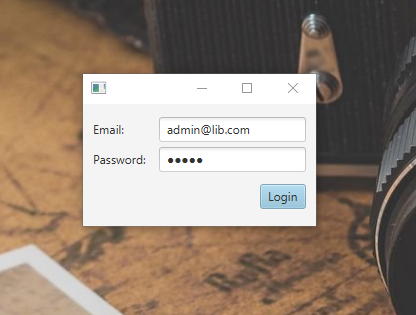
\includegraphics[width=\textwidth]{Include/Resources/FrontendScreens/JavaFX/adminLogin.png}
    \caption{Login window}
    \label{fig:ScreenshotGUIadminLogin}
\end{figure}




%%%%%%%%%%%%%%%%%%%%%%%%%%%%%%%%%%%%%%%%%
\begin{figure}[H]
    \centering
    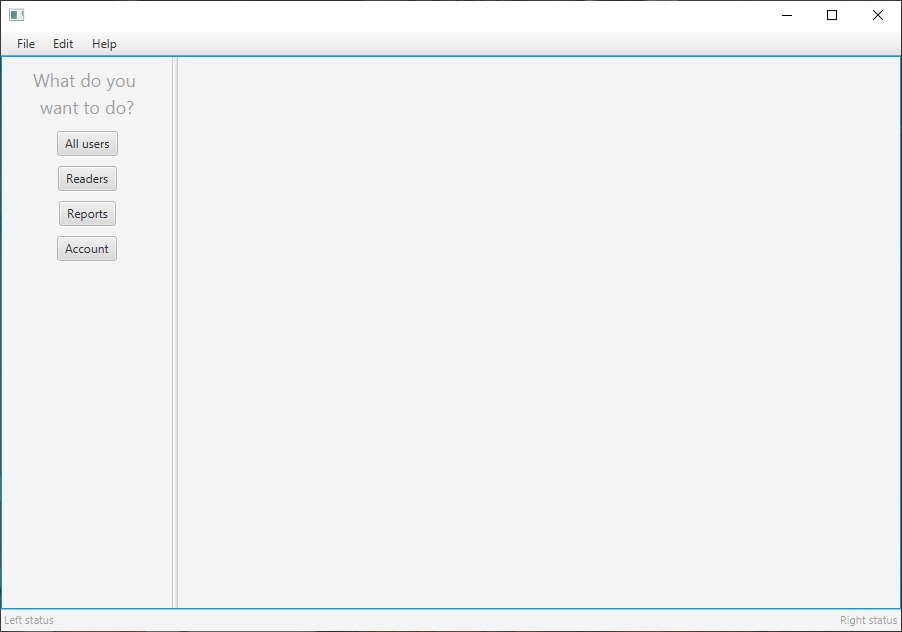
\includegraphics[width=\textwidth]{Include/Resources/FrontendScreens/JavaFX/adminNotSelected.png}
    \caption{View before selection}
    \label{fig:ScreenshotGUIadminNotSelected}
\end{figure}




%%%%%%%%%%%%%%%%%%%%%%%%%%%%%%%%%%%%%%%%%
\begin{figure}[H]
    \centering
    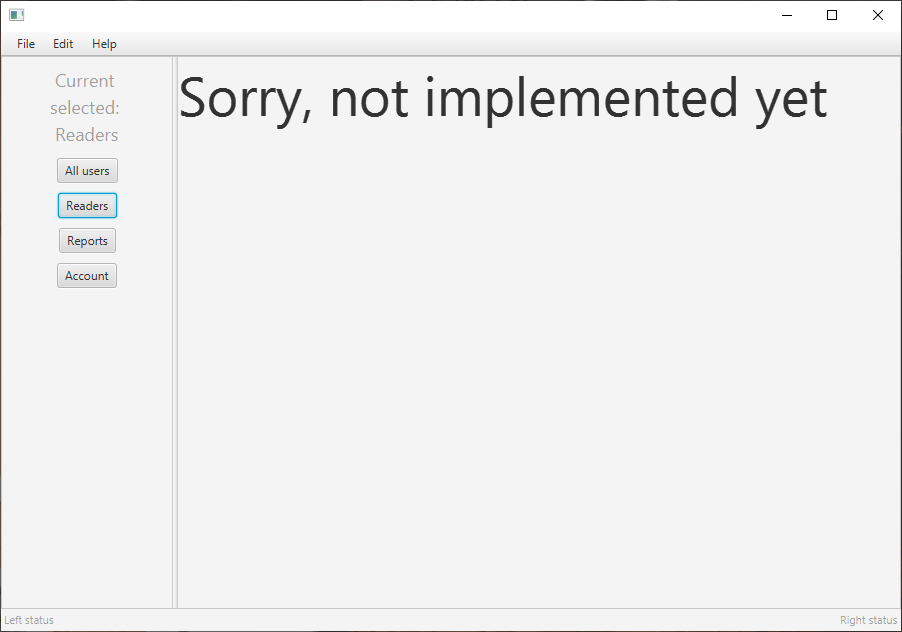
\includegraphics[width=\textwidth]{Include/Resources/FrontendScreens/JavaFX/adminNotImplemented.png}
    \caption{View of not implemented section}
    \label{fig:ScreenshotGUIadminNotImplemented}
\end{figure}




%%%%%%%%%%%%%%%%%%%%%%%%%%%%%%%%%%%%%%%%%
\begin{figure}[H]
    \centering
    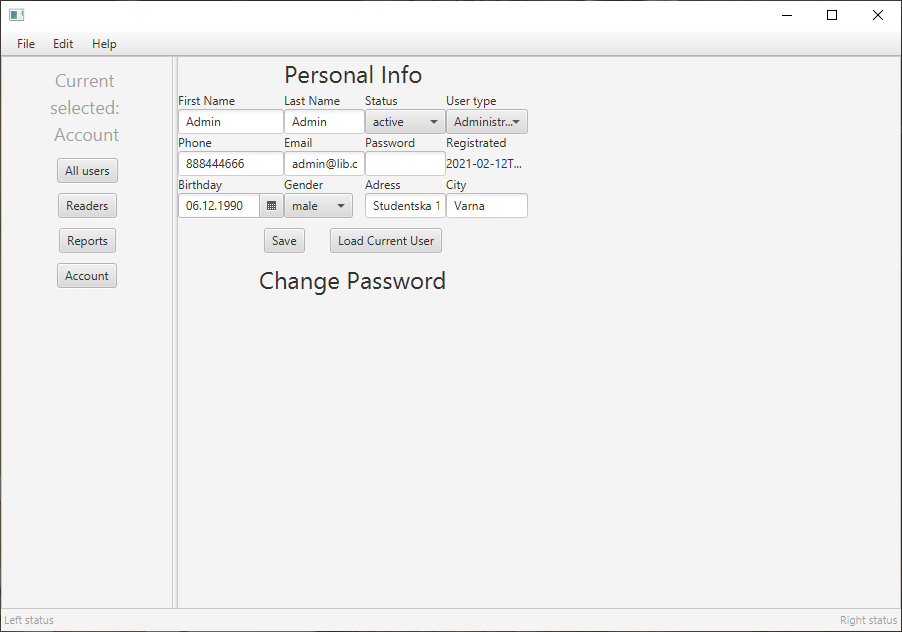
\includegraphics[width=\textwidth]{Include/Resources/FrontendScreens/JavaFX/adminAccount.png}
    \caption{Account section view}
    \label{fig:ScreenshotGUIadminAccount}
\end{figure}




%%%%%%%%%%%%%%%%%%%%%%%%%%%%%%%%%%%%%%%%%
\begin{figure}[H]
    \centering
    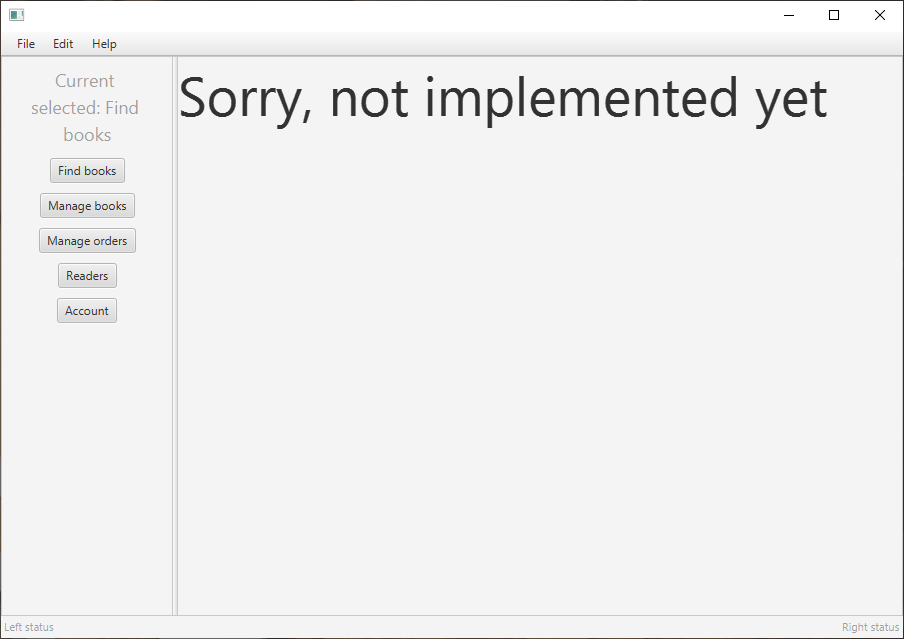
\includegraphics[width=\textwidth]{Include/Resources/FrontendScreens/JavaFX/librarianNotImplemented.png}
    \caption{Librarian sidebar buttons}
    \label{fig:ScreenshotGUIlibrarianNotImplemented}
\end{figure}




%%%%%%%%%%%%%%%%%%%%%%%%%%%%%%%%%%%%%%%%%
\begin{figure}[H]
    \centering
    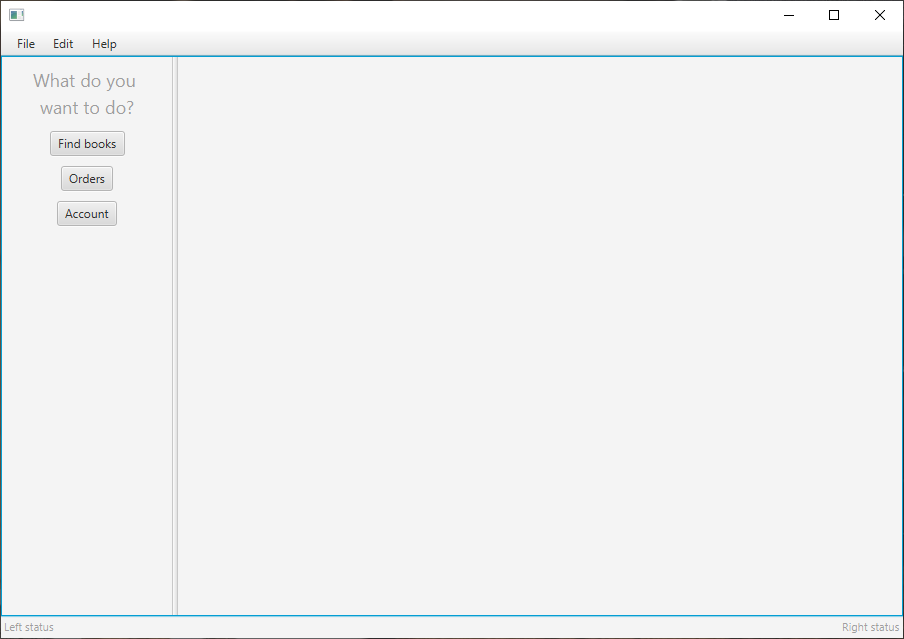
\includegraphics[width=\textwidth]{Include/Resources/FrontendScreens/JavaFX/readerNotSelected.png}
    \caption{Reader sidebar buttons}
    \label{fig:ScreenshotGUIreaderNotSelected}
\end{figure}



